\documentclass{tufte-handout}

%\geometry{showframe}% for debugging purposes -- displays the margins

\usepackage{amsmath}

% Set up the images/graphics package
\usepackage{graphicx}
\setkeys{Gin}{width=\linewidth,totalheight=\textheight,keepaspectratio}
\graphicspath{{graphics/}}

\title{Finding ``Beyond Being There'': New Communication Channels with Non-Verbal Actions}
\author[Drew Harry]{Drew Harry}
%\date{24 January 2009}  % if the \date{} command is left out, the current date will be used

% The following package makes prettier tables.  We're all about the bling!
\usepackage{booktabs}

% The units package provides nice, non-stacked fractions and better spacing
% for units.
\usepackage{units}

% The fancyvrb package lets us customize the formatting of verbatim
% environments.  We use a slightly smaller font.
\usepackage{fancyvrb}
\fvset{fontsize=\normalsize}

% Small sections of multiple columns
\usepackage{multicol}

% Provides paragraphs of dummy text
\usepackage{lipsum}

\begin{document}

\maketitle% this prints the handout title, author, and date

% Leaving this disabled for now - will want to separate it onto a different page eventually. 
% \tableofcontents

\begin{abstract}
\noindent Although it's been 20 years since the ``beyond being there'' argument was first made, most of our communication and collaboration experiences have retained their focus on recreating face-to-face interaction. In this proposal, I outline my strategy for designing interfaces that move beyond face-to-face experiences by creating new mediated communication channels that complement existing synchronous communication channels. I use shared displays to help support creating common ground among users. I illustrate these design strategies using a series of three projects: \emph{Information Spaces}, \emph{backchan.nl}, and \emph{Tin Can Classroom} and describe my current project that ties these strategies together: \emph{Tin Can Conference}. In each of these projects I trace the influence of my three major research themes: grounding, non-verbal actions, and attention as well as identify the major contributions that my work will make.
\end{abstract}

%\printclassoptions

% looks like I'm allowed to have text here, but not going to...

\section{Introduction}

% There are a few different strategies we can go with here. We could attack the beyond being there problem, and go for the "thinking about face to face" bit. Alternatively, a more general plea for shifting attention back to synchronicity - asynchronous has its issues, and we still (rightfully) privilege real time encounters. The motivating metaphor here being the weirdly object-centric models of asychronous encounters, not people-centric models.

% Some other related themes:
% - stages
% - channels
% - attention
% - text v audio
% - power relationships / confidence?
% - ???

% The core question is what do my systems encompass and lend themselves more to. Clearly they're all synchronous experiences, not async. So that's fine. 

% Okay, here's what we'll do - leave the sync/async pendulum stuff to the background section as a way of framing the history of system design in this space. Focus on the beyond being there story for the introduction.

\begin{marginfigure}
	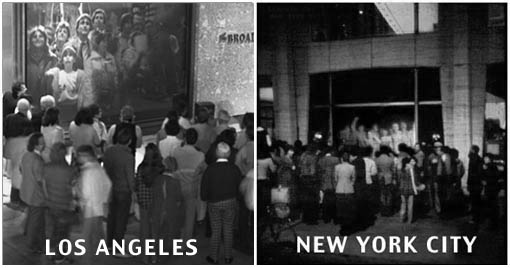
\includegraphics{figures/hole_in_space.jpg}
	\caption{Photos of the Hole in Space exhibit sites in Los Angeles and New York City.}
	\label{fig:hole-in-space}
\end{marginfigure}

\begin{marginfigure}
	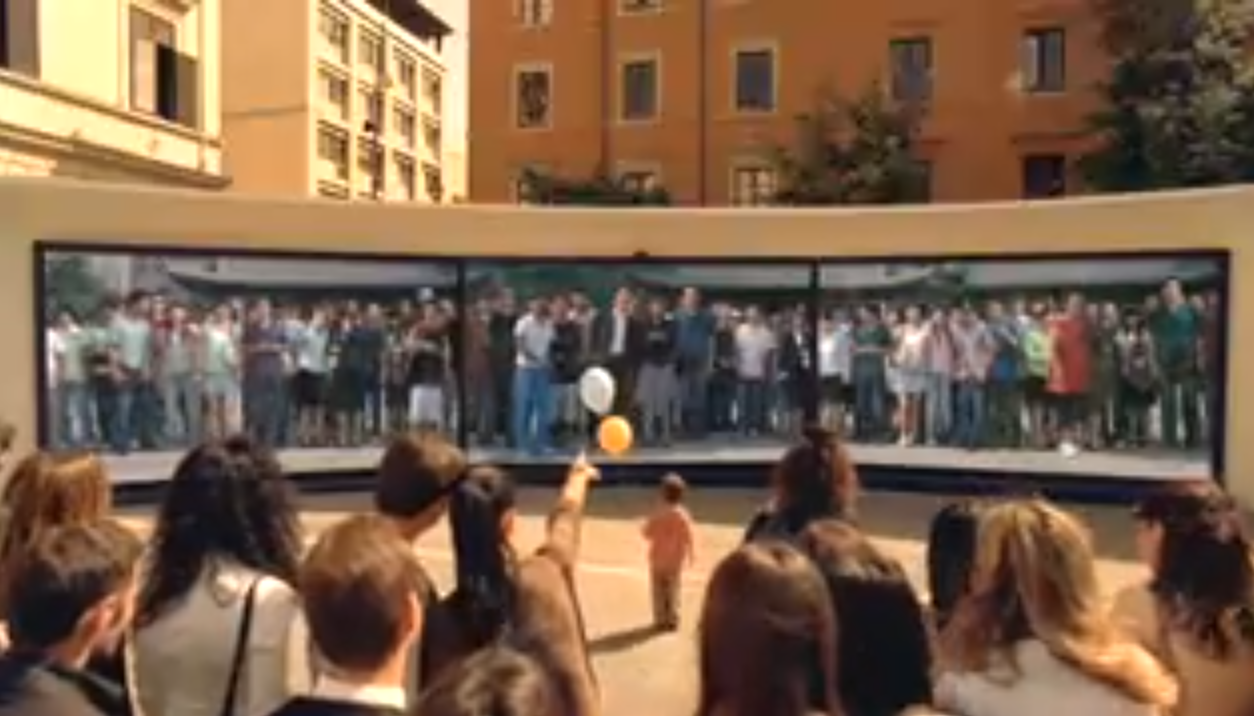
\includegraphics{figures/cisco-telepresence.png}
	\caption{Still from a Cisco Telepresence advertisement, centered on connecting an Italian piazza with a Chinese square with a seamless window.}
	\label{fig:cisco-telepresence}
\end{marginfigure}

\begin{marginfigure}
	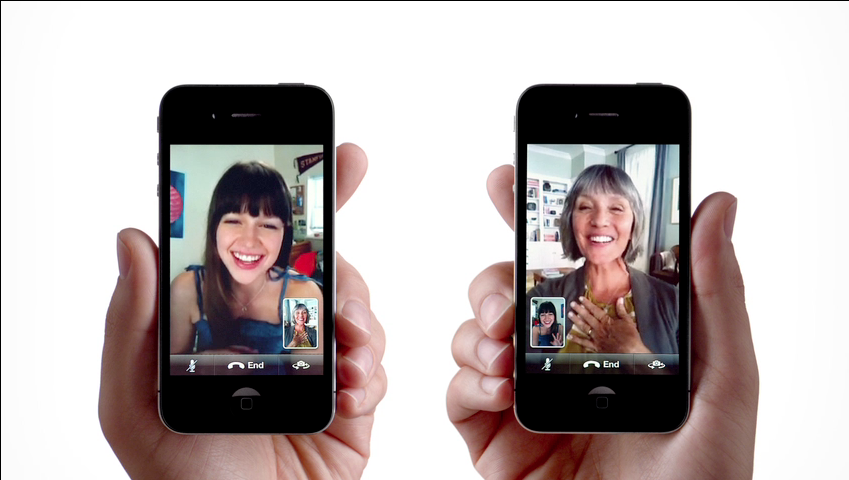
\includegraphics{figures/iphone-face-to-face.png}
	\caption{Still from an Apple advertisement demonstrating the Facetime feature to enable mobile video conferencing.}
	\label{fig:facetime}
\end{marginfigure}


As researchers first started to build technology to help us communicate with other people at a distance, a consensus on what the goal should be quickly arose: computer mediated communication systems should focus on recreating the experience of being face-to-face with another person. The best system, in this model, is one that seems to disappear, in same way the best window makes us feel like there's nothing between us and the other side of the glass. Since the early 1970's, it has seemed like we were on the cusp of making distance disappear and moving all our communication to mediated channels. \citep{Egido:1988vq} And yet, like the paperless office \citep{Sellen:2001uk}, we are left wondering if perhaps the persistence of a preference for face-to-face communication represents a similar failure to recognize both the subtle qualities of what we're trying to replace and the true potential of what we're trying to replace it with. 



% I want to be able to cite the commercials, but it's a nightmare finding any information about them that might make them citable like where they appeared, when they appeared, who directed them, etc.

There's an undeniable magic to the pursuit of recreating face-to-face communication at a distance. This magic is most poetically captured in the famous ``Hole in Space'' \citep{HoleinSpace:1980vn} piece, visually and audibly connecting a storefront in Los Angeles and New York in a way that seemed to make distance disappear. This same magic continues to motivate modern communication tools from major companies; Cisco and Apple, among others, have played on this utopian vision of a future where distance is no barrier to communication in their commercials for so-called ``telepresence'' tools and mobile phones with cameras, respectively. This vision is not simply aspirational, either. Tools to communicate with physically distant people either with audio alone or with an added video connection play a role in the daily lives of millions of people. This desire to experience ``being there'' with someone else is powerful and compelling. 

It is not, however, the only way to approach this problem. In their famous paper, \citet{Hollan:1992tz} suggest an alternative approach which they named ``beyond being there''. They argue that seeking to recreate the experience of ``being there'' was in a way an abdication of our responsibility as designers that left an important design space un-explored. In particular, they urge us to think less about ways to minimize the experience of mediation in communication, but to look instead for ways that mediation can add value to interactions. To take this perspective seriously, we need to shift away from a view of face-to-face interaction as being always better than interactions mediated by technology and instead think critically about potential limitations and challenges with face-to-face interaction and potential benefits that mediation can offer. 

% think about listifying this section

Many of these challenges are common sense, even if they are frequently forgotten when people argue for recreating face-to-face experiences. Face-to-face communication requires relatively explicit turn-taking; multiple speakers in a group make them all largely unintelligible. In mediated environments like chat, simultaneous conversation threads can easily co-exist for long periods of time. There are major identity implications to face-to-face communication. It is difficult to conduct any face-to-face communication without revealing significant information about your identity. In mediated contexts, there are techniques ranging from anonymity to pseudonymity to limit identity disclosing information. Participation in non-mediated interactions is ephemeral, while mediated interaction can easily be archived and represented either in context or after the fact. Participation in face-to-face situations can be limited by confidence, but mediated participation tends to be more disinhibited. \citep{Siegel:1986ve}

% is this a second order effect?
% For a variety of reasons, the power dynamics in social situations are more easily subverted in mediated environments. 

All of these challenges and differences between face-to-face interaction and  mediated communication (broadly construed) represent a major opportunity. In my work, I focus on building systems that add new mediated communication channels to existing familiar communication experiences. The goal of these interventions is to create environments where people have ways to express themselves non-verbally in addition to whatever existing communication channels exist. In some of my work this means building systems to augment face to face situations that are not traditionally mediated at all; in other situations, I look at already-mediated experiences and add new kinds of non-verbal communication options. By adding mediated communication channels to other existing channels, we can focus on the affordances of each channel to let it do what it does best.

% Part of what's attractive about mediated communication systems is that there is a tremendous variety of ways to design and use them once we set aside a desire to recreate face-to-face interaction. Although in this section I've contrasted mediated communication with face-to-face communication in a way that might imply that mediated communication systems are somehow monolithic and self-similar, the survey of related systems in the section to follow will illustrate the tremendous range of potential systems in this space and demonstrate how thoughtful designs can have widely varying impacts on the experience of communication or collaboration. 

My work takes this general design of adding new communication channels in a few different directions. In this proposal, I will describe my past work looking at meetings in virtual worlds, audience-speaker interaction in presentations, and classroom discussions, as well as lay out my design for a system to support face-to-face meetings with remote participants. These research contexts vary both in the numbers of simultaneous participants, as well as their geographic configuration; in some cases everyone is in the same physical space, in others they are all remote. In my future work, I will study a hybrid of those two situations.

Across this set of projects, I explore three major research themes:

\begin{description}
	\item[Grounding]{My work uses shared displays in a variety of different capacities. I contend that these kinds of public displays can play a powerful role in helping to ground, in the \citet{Clark:1989uc} sense, a conversation. In particular, shared displays can provide ways to non-verbally acknowledge discourse presentations. By their very shared nature, the contents of shared displays might accelerate the creation of common ground. The different ways that these shared displays operate in my work helps provide insight into both particular design techniques to support grounding as well as the broader discussion around how common ground operates in mediated communication contexts.}
	\item[Non-verbal actions]{As a result of the drive to create a sense of ``being there'', mediated interaction systems failed to consider the ways that we communicate non-verbally, assuming that higher fidelity video and audio would be sufficient to capture that communication. I contend that our non-verbal actions in the physical world are a critical component of body language, and when creating mediated channels we should strive to create new vocabularies of action that enable people to communicate non-verbally. In much the same way that in a shared physical space we can observe people interact with objects around us, so too should people's actions in mediated systems be visible and part of supporting a sense of presence and awareness.}
	\item[Attention]{Adding communication channels forces us to decide how we manage our attention. Which channels do we attend to? How is our attention made visible to others, and how does it affect their impressions of us? Furthermore, how we decide which channels are appropriate for which kind of communication? Although attention is not an inherent design issue, understanding  how people think about and enact attention in situations with multiple available communication channels is critical to designing appropriate options and understanding the practices that evolve around them.}
\end{description}

The contributions of this work will be on two levels. First, by creating and deploying interfaces with particular properties, I can provide concrete guidance and insight about particular specific design strategies and interfaces. This is valuable for designers and researchers thinking about how they design this variety of communication systems, a space which based on my interactions with sponsors is increasingly relevant. I will also contribute to the broader discourse about the three research themes laid out above. In each case there are both broader theoretical contributions to be made as well as specific findings that contribute to scholarly discussions about these issues.




% I have focused my work in a number of ways. Although many of the interfaces proposed as being ``beyond being there'' in their original paper are asynchronous systems, I focus exclusively on synchronous experiences -- co-temporal experiences where participants are communicating and using a system at the same time. I focus primarily on medium sized groups and crowds. Although the groups are always interacting co-temporally, they are sometimes all in one physical place, and sometimes geographically distributed. 

% It can be difficult to describe exactly what the contributions of design focused research can be. In my work, I see two major categories of contributions. First, by building systems and testing them \emph{in situ} I can provide concrete guidance about particular specific design strategies and interfaces were used by users in practice. This is valuable for designers and researchers thinking about how they design non-verbal communication systems in their own work. I also engage with broader theoretical questions about attention, signaling, grounding. By contributing to these larger discourses with specific findings in studies of my own systems, I hope to contribute to broader discussions in computer mediated communication. 

% gotta really settle on what my themes are going to be here. current list is:
%  - attention (solid)
%  - signaling (erm - what is this exactly?)
%  - grounding (I like)
%  - 


% It can be difficult to describe exactly what the contributions of design focused research can be. Is making something that people describe as useful a sufficient outcome, or should we expect more? I conceive of my research as being a kind of design cartographer. Given the design space I outlined earlier, I try to identify and describe compelling and effective design strategies. Beyond the specific contributions of design elements that are valuable, I step back from the specifics of each system and theorize about general themes that are relevant to any sort of design work in the space. In this case, these are themes like stages, performative attention and contribution, norms, power dynamics, and grounding. By contributing in both of these ways, I seek to support designers and researchers working both with modern constraints as well as contribute theoretically to ways of thinking about design of co-temporal mediated experiences that will give us the tools to think about as-yet-unimagined design spaces.

% At that scale, I find that the benefits of being face-to-face are strongest and successful interventions are quite difficult to produce. (Leave the research strategic points for later?)

% talk about general themes + backchannels

In this dissertation proposal, I will start with a survey of relevant related systems, as well as briefly touching on experimental, theoretical, and methodological work that plays a significant role in my work. Then I will describe the arc of my past work with a focus on my final project: Tin Can. Finally, I will describe in general terms the contributions and potential impact of this work.

% need to do a bunch of reference-finding for this section. find people talking about the history of telecommuting, early telephone motivations, telegraph, video conferencing, etc to back this all up. 
% try to dig up that reference where people talk about early claims about telecommuting and teleconferencing...

% TODO the core problem with this introduction is that it never really talks about backchannels or side channels or anything. I specify the domain, but not my primary design strategy. It really should be more about that. Another way to put that is that this is not saying "problem X -> solution Y -> justification Z". I could certainly write something like that, and it might be productive. We'll let this percolate (and maybe get someone in the group to read it and see) and come back to that question. 

\section{Background}

Designing new systems for collaboration and communication, as opposed to studying existing systems, has long been a major stream of HCI and CSCW research. This section will summarize the most salient past work in this area, although little of this work is recent and responsive to the significant shifts in the way people use technology to communicate, collaborate, and play. 

For a variety of reasons, there has been somewhat of a shift in interest away from the kind of co-temporal interfaces and experiences I create towards building and studying systems for asynchronous experiences between much larger numbers of people. The advent of research on mass collaboration systems like \emph{Wikipedia} (e.g. \citep{Kittur:2007up}) and ``crowd sourcing'' (e.g. \citep{Bernstein:2010wk}) is part of a larger shift away from what was once the center of gravity of systems research. This shift is a natural response to changes in both technology and the common experience of modern collaborative technology users in a web-oriented world where asynchronous interaction became the norm.

In this work, I argue that we should not neglect the design of synchronous interfaces and experiences for small groups. We should think not just about how to marshal large numbers of people, but about how small groups of people who know each other work, recognizing that much of that work happens face-to-face or co-temporally while geographically distant. It is not effective to treat these interactions as a simple increase in tempo on asynchronous interactions. In synchronous systems, experiences of presence and understanding how we are perceived (and can control those perceptions) by others are quite important. In asynchronous systems, these issues are minimized; we experience others through their actions on shared objects like documents.

% In my work, I seek to create richer representations of people and better-support person-person interaction instead of person-document-person interaction. 

To further motivate my work and situate it within the larger space of systems design research, I survey related work in this section. The work is organized into two major themes: adding new communication channels and ways to help people reflect on the participation of themselves and others.

% TODO think about whether to add in a chunk about theoretical perspectives here. Ultimately in the final dissertation there will need to (probably) be a chapter or serious chunk of one laying our theoretical perspecives on grounding, attention, and non-verbal actions. But I don't really want to have to do that now.


\subsection{Channels}

The primary focus of my work is on designing systems that add new communication channels and understanding how those channels operate in contrast to existing channels. In this section, I will present related work that addresses some of these questions.

The work most directly related to these questions comes from research into so-called ``backchannels'' in presentation and classroom settings. \citet{Yardi:2006uk} describes how a chat-based backchannel operates over a semester in a classroom, \citet{mccarthy_digital_2004} describe a similar approach at a conference. Backchannels can also be considered a potential part of non-event-oriented contexts too, like long-term co-working among small groups. \citep{Huang:2003ef} Backchannels are not just focused on co-located groups, however, and \citet{kellogg_leveraging_2006} (among others, e.g.  \citep{Yankelovich:2005bx}) has addressed how text and audio backchannels can operate in distributed contexts. This is the main literature that I hope to contribute to. Although past work has addressed in general terms the different ways people use backchannels, it has not sufficiently explained the complicated issues around channel selection, attention, distraction, and identity. Furthermore, in my work I try to move beyond just adding new text or audio channels by adding other kinds of non-verbal actions.

\begin{marginfigure}
	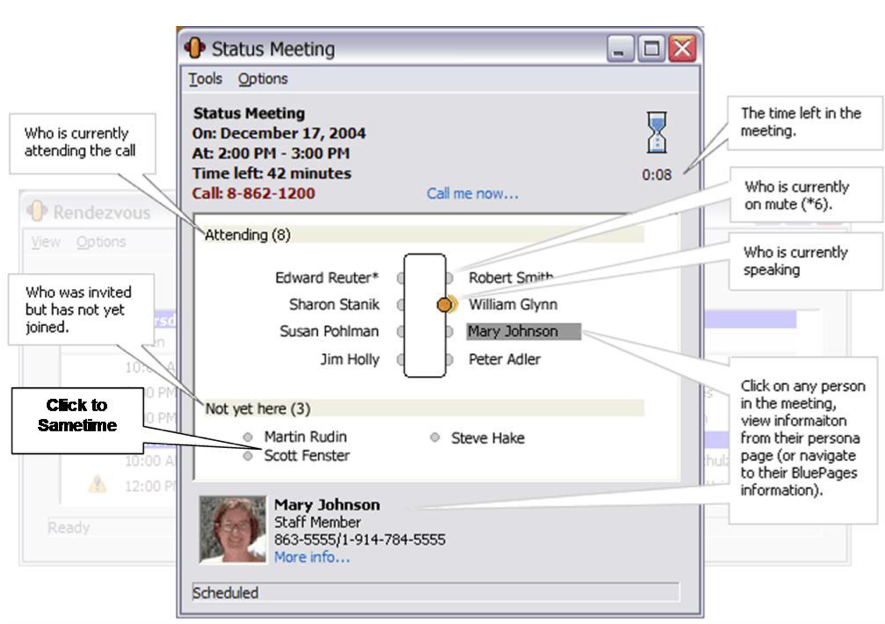
\includegraphics{figures/kellog_social_proxies.png}
	\caption{Screenshot of a particular Social Proxy for promoting a sense of awareness of other meeting participants, from \citep{kellogg_leveraging_2006}.}
	\label{fig:social-proxies}
\end{marginfigure}

\begin{marginfigure}
	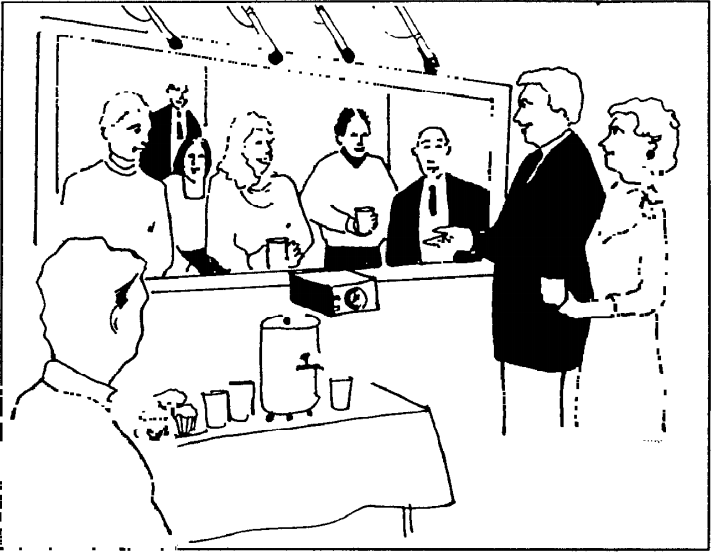
\includegraphics{figures/videowindow.png}
	\caption{Diagram of the VideoWindow scenario for connecting two work-place social spaces, from \citep{Fish:1990fn}}
	\label{fig:videowindow}
\end{marginfigure}


Much of the work on creating shared media spaces, driven by experiments at PARC in the late 1980's and early 1990's is salient to my work. Although in some cases this work focused on creating new primary channels, researchers quickly became attuned to problems of privacy and attention because such systems always co-exist with face-to-face communication, in much the same way they do in systems I design. The earliest work at PARC \citep{Olson:1991vz} focused on creating flexible video connections between offices and conference rooms. Subsequent work focused less on a phone-call-like model where connections are created and ended and shifted towards creating spaces with different affordances. Sometimes these involved connecting multiple individuals together, as in CAVECAT \citep{Mantei:1991ww}; other times researchers focused on creating a long term persistent video connections in common areas of distributed research groups in the VideoWindow \citep{Fish:1990fn} project.

Over time, attention shifted more towards a taking advantage of the possibilities to do more than just create ``being there'' experiences. Some researchers experimented with audio-only spaces \citep{Hindus:1996cn}, finding that video was not required to create a sense of connection and space for users, but that the properties of audio did require audio-specific etiquette and coping strategies for the system to be useful. iCom represented a particularly rich design perspective on connecting spaces  \citep{Agamanolis:2003wc}, recognizing that awareness need not be limited to visual awareness, but can extend to information awareness which can be productively embedded in a media space. This embodies the ``beyond being there'' model best of all the work in this research stream: not just trying to create a transparent window between remote spaces, but making something better than a window could be.

% \begin{marginfigure}
% 	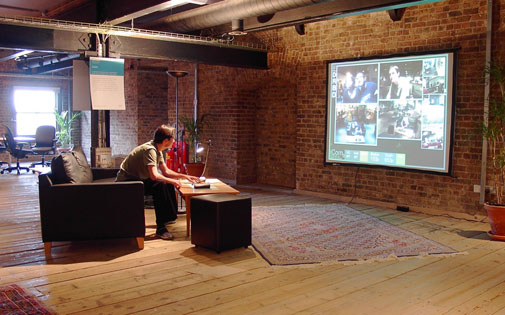
\includegraphics{figures/icom.jpg}
% 	\caption{Photo of one end of an iCom connection, showing multiple video streams and metadata along the bottom of the screen, from \citep{Agamanolis:2003wc}.}
% 	\label{fig:icom}
% \end{marginfigure}

\begin{marginfigure}
	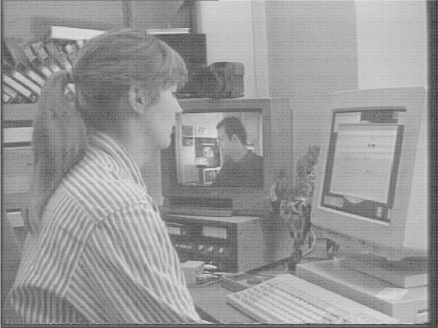
\includegraphics{figures/CRUISER.png}
	\caption{Photo of a CRUISER station installed in an office, from \citep{Fish:1992vz}.}
	\label{fig:cruiser}
\end{marginfigure}

\begin{marginfigure}
	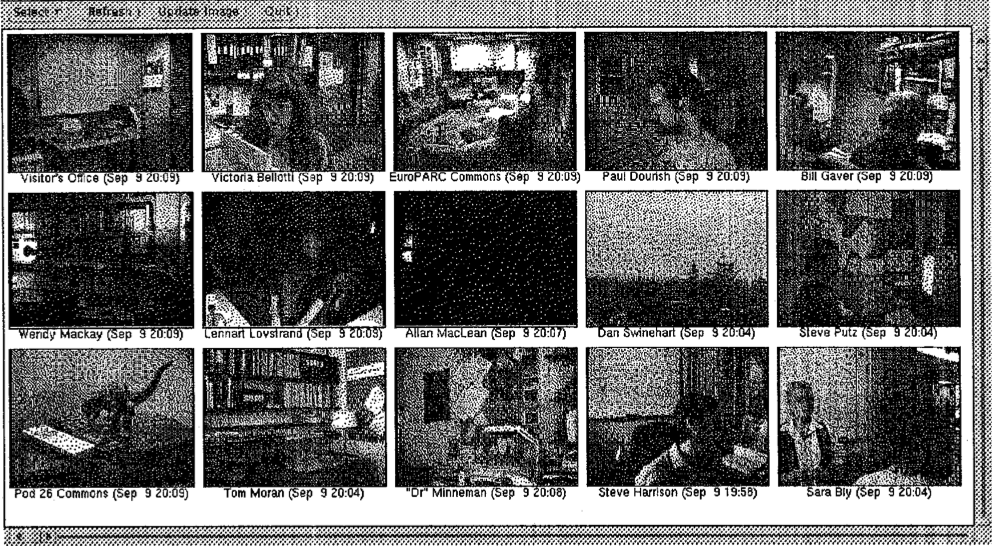
\includegraphics{figures/portholes.png}
	\caption{Screenshot of the Portholes interface, showing periodic stills from a wide range of environmental cameras in an office environment, from \citep{Dourish:1992fu}.}
	\label{fig:portholes}
\end{marginfigure}

\begin{marginfigure}
	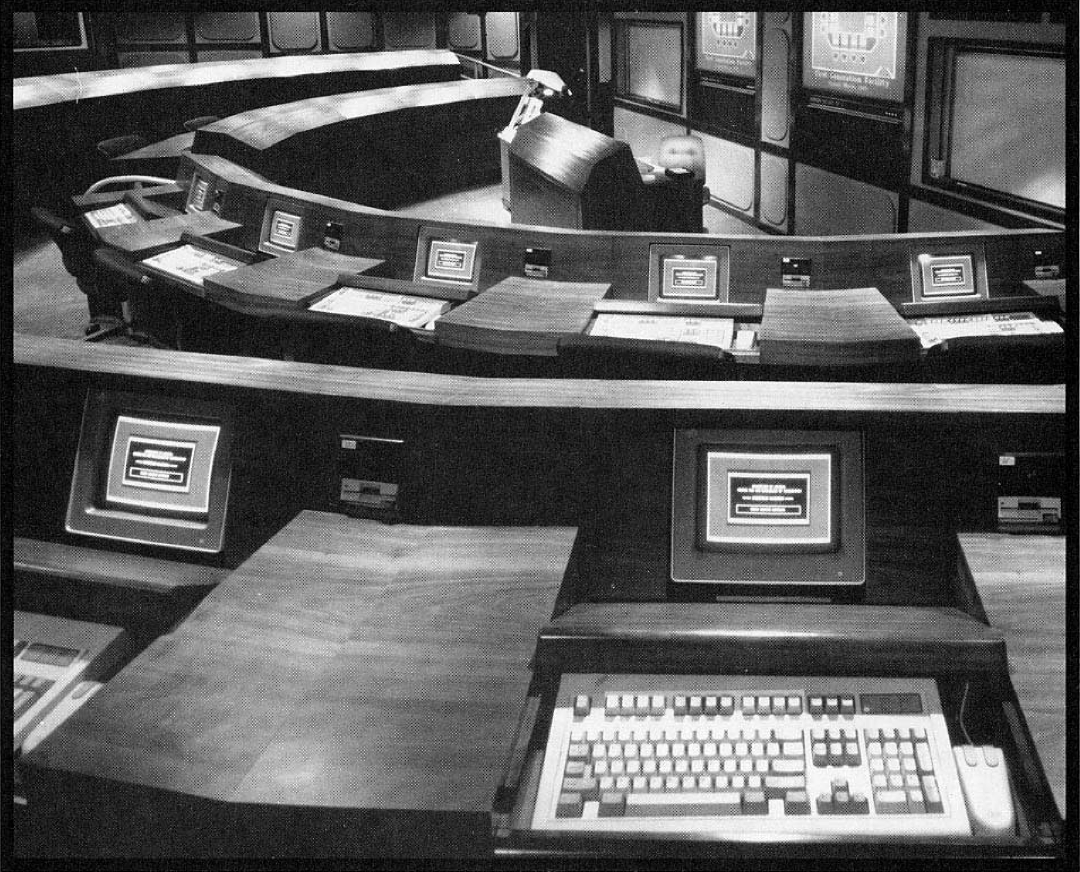
\includegraphics{figures/nunamaker_gdss.png}
	\caption{Photo of a GDSS space, from \citep{nunamaker_electronic_1991}.}
	\label{fig:gdss}
\end{marginfigure}


% also cite karrie's 
% (For subsequent, more artistically inclined approaches to this design space, see Karrie's blah blah, get a nice figure in here for that.)


Serendipity also evolved as an important part of sharing an office environment that was not present with most media space systems. Portholes \citep{Dourish:1992fu} addressed this explicitly by giving people a broader view of remote spaces instead of focusing just on main channel interactions. While my work is not concerned with serendipity, this kind of visual side channel carries important awareness information in much the same way that the side channels in my systems add important contextual information to an interaction. CRUISER \citep{Fish:1992vz} offered non-verbal ways to signal a desire to emulate some of the office hallway etiquette for signaling a desire to drop in and chat informally, without the explicitness of placing a call. The addition of moves like ``cruise'', ``glance'', and ``visit'' are similar in approach to the non-verbal actions at the core of my work like voting in backchan.nl, promoting ideas in Tin Can, or moving around the field in Information Spaces. 

Early media space researchers proposed a distinction between ``formal'' systems from ``informal'' systems. \citep{Olson:1991vz} While most of the work discussed here (and much of my own work) tends towards the informal side of that continuum, there are some formal elements in my work. This formality manifests most strongly in Group Decision Support Systems research. These systems (exemplified by the work of Nunamaker \citep{nunamaker_electronic_1991}) provide prescriptive systems to support particular brainstorming, decision making, outlining, and voting schemes or policies. In the typical GDSS configuration, each participant has their own computer and interacts with shared structured data in some way, like submitting a new idea or voting on a proposal. The lack of consistent results in comparative work in this area \citep{Dennis:1988ww} illustrates the importance of focused design analysis to contextualize findings; it is not useful to view all brainstorming systems as equivalent and comparable in analysis, and I hope that my work will illustrate how the subtleties in interface and approach can have big impacts on outcomes that help explain some of the contradictory results in past GDSS work. Work in this space also raises serious questions related to attention that their work largely fails to address. In fact, in many situations they advocate for largely shutting down pre-existing primary communication channels to focus on the structured, mediated alternative.

% go hunting for a desanctis and/or poole piece that's not focusing on AST specifically? also can hit berg if we want, but it feels like a bit of a distraction at the moment.

%, they also produced a nice taxonomy of the kinds of tools that would be useful for distributed collaborative groups: synchronous versus asynchronous communication and open processes versus focused processes, a distinction 


% there's a funny note in the portland paper about how they want to shift away from meeting augmentation to async and task coordination. Funny how times change.

% now summarize. 


% going to want to bring up media equation or whatever that book is called. Cliff Nass. 




% thundewire is just audio, basically a single-channel mumble. not so much about results as describing practices that evolved. 
% portholes is ambient awareness about remote places, not live interaction. cut it?
% videowindow is just like hole in space - audio/video fixed in space

% also mention virtual world stuff? MASSIVE might be worth a quick ref

% "shared media systems"

% - video projects like thunderwire + portholes
% - videowindow


% organize the work in this space 
% projects to talk about:
% - voiceloops
% - backchannel literature
% - social proxies
% - mention conferencing apps
% - Nunamaker
% - zephyr?


% \subsection{Theoretical Perspectives}
% thinking about leaving this out

% stuff from cscw paper:
% systems for reflection
% - second messenger
% - "social mirror" (Karahalios) also bergstrom
% - Meeting Mediator
% 
% systems adding new channels
% - (all the backchan literature: yardi, mccarthy, huang, kellog, yankelovich)
% - do a section on nunameker's work and why it's weird
% - 

% - we'll want to at the very least nod to thinks like voiceloops, and all the audio/video stuff like portholes and thunderwire and that kind of thing. farm my generals reading for that part.
%


% theoretical perspectives
% - practice lens?
% - ethnomethodology? 
% - re-farm wanda's reading list to see what else I can pull from there.

%
% We'll need to do a little organization here. Obviously, farm the references from the Tin Can Edu CSCW paper + backchan.nl paper. We'll need more, ofc, but it's a start. I suspect there will be some ways to separate out systems that allow communication versus those that simply reflect on a main channel. Maybe it's about whether the system itself is a single channel, multi channel, main channel or side channel? 

% write a methodological section here about why it's useful to study this with design work

\subsection{Reflection}

\begin{marginfigure}
	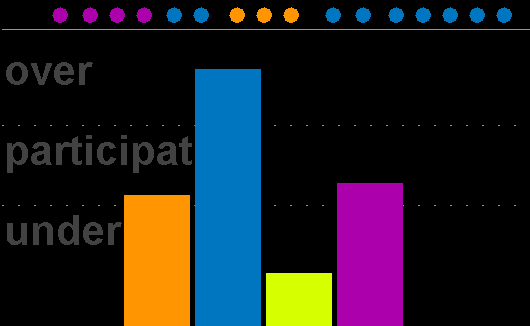
\includegraphics{figures/second-messenger.png}
	\caption{Screenshot of a Second Messenger participation bar-chart, from \citep{DiMicco:2007ie}.}
	\label{fig:second-messenger}
\end{marginfigure}

% \begin{marginfigure}
% 	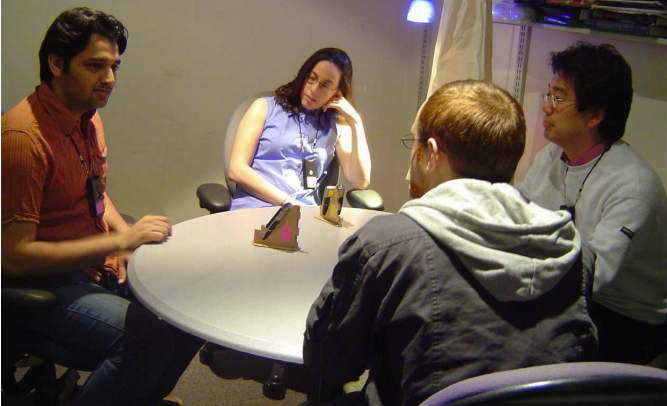
\includegraphics{figures/meeting_mediator.png}
% 	\caption{Meeting mediator.}
% 	\label{fig:meeting-mediator}
% \end{marginfigure}

\begin{marginfigure}
	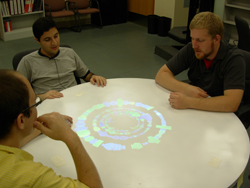
\includegraphics{figures/conversation_clock.png}
	\caption{Photo of Conversation Clock in use, showing relative participation histories from each conversation participant, from \citep{Bergstrom:2007je}.}
	\label{fig:conversation-clock}
\end{marginfigure}

\begin{marginfigure}
	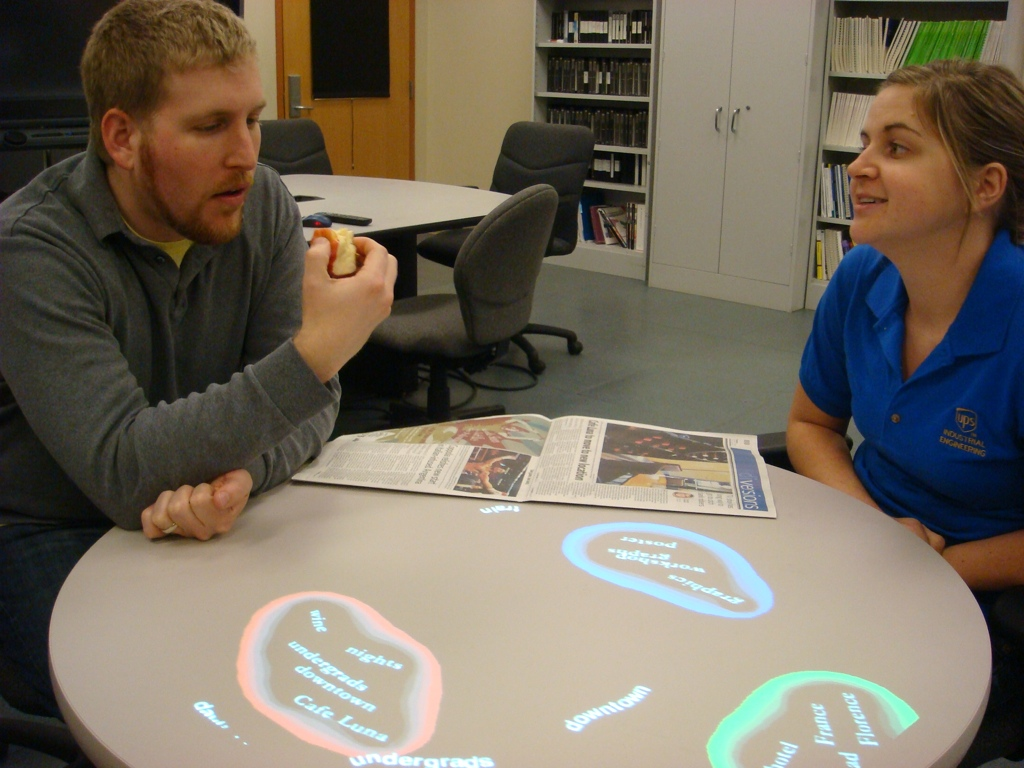
\includegraphics{figures/conversation_clusters.jpg}
	\caption{Photo of Conversation Clusters, detecting audio themes and displaying them in visual clusters on the table-top display, from  \citep{Bergstrom:2009fe}.}
	\label{fig:conversation-clusters}
\end{marginfigure}

\begin{marginfigure}
	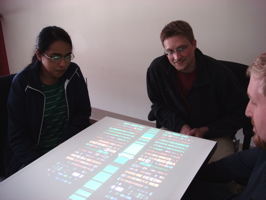
\includegraphics{figures/conversation_votes.jpg}
	\caption{Photo of Conversation Votes, showing voting history among conversation participants on the table-top display, from \citep{Bergstrom:2009ej}.}
	\label{fig:conversation-votes}
\end{marginfigure}


Understanding how we present ourselves to others has been a topic of sociological inquiry for quite some time. Although many of the insights of scholars like \citet{goffman_presentation_1959} about how we communicate and interpret information about who we are and how we want to be treated are still relevant, the information that is available about people has changed substantially. In some of the examples in this section, designers have added some new bit of information about people to a face to face discussion; in others, we don't have any of the traditional information we would get from being face to face with someone and rely on new types of signals (like the non-verbal actions I propose) to create a sense of people around us. Part of what sets mediated communication apart is the ability to accumulate behavioral histories and represent and reflect those histories to ourselves and others.


My work is substantially inspired by the work of \citet{DiMicco:2007ie} on the Second Messenger project. In this project, participants in a group discussion were presented with a constantly-updating bar-chart visualization representing the relative amount of time they had talked during the discussion. They found that while people who over-participated without a visualization tended to moderate their participation when the visualization was present, people with low participation did not participate more just because others were participating less. Meeting Mediator \citep{Kim:2008ip} took a similar approach, but focused on situations where groups of two people could see each other and had to interact with another group of two people who they could only hear. Using a different visualization, Kim found that groups were more interactive with the system than without, although there was not a correlation with group performance. 


Bergstrom has done a series of projects that adopt a similar design strategy. Conversation Clusters \citep{Bergstrom:2009fe} pulls topics from an audio conversation and presents them in clusters on a table-top display. Conversation Clock \citep{Bergstrom:2007je}, like Second Messenger and Meeting Mediator, visualizes conversation participation, but uses a timeline metaphor instead of a aggregative metaphor. Conversation Votes \citep{Bergstrom:2009ej} lets uses discreetly vote about the progress of a discussion, and displays anonymous votes on a table-based display. \citet{Bergstrom:hu} describes this design space as ``social mirrors''. 

% sneak in a \citep{visiphone} here?


% MATT TODO FIX THE MIDDLE OF THIS PARAGRAPH IT'S AWFUL
These are all examples of the accumulate and reflect design strategy, where the system tracks some aspect of behavior: verbal participation in the case of Second Messenger and Meeting Mediator, discussion topics and group attitudes in the case of Bergstrom's work. The systems then present that information back to the individual or group and the hope is they will use it to reflect on and potentially adjust their behavior. Much of my work uses this strategy in different ways as a way of making non-verbal actions persistent and visual in a way that makes them more visible and long-lasting than momentary events.  Furthermore, all of these projects have an element of grounding to them. By presenting this social information on a shared display (as in my work), it is made salient to the discussion in a way that private displays cannot.

% cite things like last.fm, goodreads, etc in this space?


% \subsection{Identity}

% maybe this whole section is dumb.
% how often do I really deal with this? It's clearly part of the second life work, but not at all part of backchannl, and only a little a part of the Tin Can series. Erm. Move on for now and double back. 

% Many other projects have focused on how peoples' identities are presented. In most of these pieces, there is no face-to-face element, which drives the researcher's interest in developing compelling alternative options that can richly communicate who someone is in a mediated space. Many informal and practical options are in common use; displaying an icon or image chosen by someone and a pseudonym to represent themselves is a widely used design strategy in social applications throughout the internet. These spaces for self expression are frequently augmented by systems that aggregate someone's behavior in that space. This is much like the reflection techniques, but are usually summarizing events beyond any single person's experience. The community site StackOverflow \citep{stack_overflow} provides a particularly rich example of this strategy.

% screenshot a wow forum, stackoverflow, 

% These techniques feel thin compared to the richness of face-to-face interaction, and researchers have developed a number of alternative approaches. Donath's work on data portraiture in a variety of 



% link to things like Ros' work in terms of augmenting face to face interaction with extra information? Or go back to steve mann's cyborg stuff?

% need a paragraph here that's more about the identity side of things. not sure what that will be. chat circles, perhaps? talking in circles? (whichever one had that intersting voting shapes thing)

% how to fit in social proxies and social translucense



% Other potential bits we could fill in here...
% We could spend some time with social translucense
% We could look at non-vebal actions as a space
%	start with Greenbergs stuff, but really look all over for groupware/collaborative tools that had some action to them. Will find some of that in the CVE literature, which might be easy to find
% I don't talk at all about theory stuff here. Could do the spiel about shared displays and grounding, but I'm not sure how critical that is going to be ultimately.
%
%
%  One other strategy is to think about the three research themes: grounding, non-verbal actions, and attention, and go on a hunt for good literature about each of those. 


\subsection{Translucence & Awareness}

This work owes a clear debt to the work of Kellogg and Erickson on social translucence. Their work intersects with my action and grounding themes. \emph{Social translucence} is a design strategy that aims to create ``digital systems such that people's presence and activity, made appropriately perceptible, will create accountability and more easily coordinated action'' \citep{erickson_kellogg_2000_look_it_up}. They call their example systems designed for this purpose ``social proxies'' that use ``abstract visual representations ... to portray information, in addition to contextual information provided by the other common traces of user activity in mediated communication environments (e.g. persistent conversation).'' In each of their projects (Babble, Loops, ???) \citep{get_good_refs_for_these}, they seek to promote a sense of ``collective awareness'' where each person using the system has a sense of the actions of others in the system and appreciates that this awareness is mutual. 

We share an interest, in my terms, in how we can construct meaningful actions in mediated social spaces and how we can understand how public displays can help ground collaborative and discursive processes. As Erickson and Kellogg point out, this has been a topic of interest both direct and indirect for quite some time in the systems literature. \citep{some_other_stuff_here_that_they_cite}. We can also look to earlier work on collaboration spaces, like \citep{something_good_from_greenburg} and \citep{tabletop_stuff} or \citep{some_big_collaboration_room_thing}. I see my work as a continuation of their early work. Although there are many similarities in terms of findings and design strategies, I will focus here on the points of difference as a way to clarify the contributions of my work.

Although Erickson and Kellogg are particularly concerned with what is made visible and what is kept private (the difference between, in their terms, \emph{transparency} and \emph{translucence}), this is a point of divergence between our work. Although I agree with their analysis of the value of considering what actions should be made visible and what should be concealed, it is not a main focus of my analysis. In my work, reading is essentially always invisible and any other action is visible. This is partially a response to their suggestion that it is ``important that participants were aware of the others' awareness of [the properties of the system]''. In other words, if you don't know which actions are public and which are private, it diminishes the value of translucence as a design strategy. In their work, they tend to rely on physical metaphors to communicate the visibility properties of a system. This is a sensible strategy, but I feel this limits the kinds of experiences we can craft. In my work I tend towards not including invisible actions and instead create completely transparent spaces with carefully selected actions that are worth being visible. This is possible partly because the group sizes in my work are smaller than in the main examples they propose, and it's feasible to show all actions without it being overwhelming. 

They share a number of specific design findings that complement some of my experiences designing similar systems. They describe three approaches to visualizing activity: realist, mimetic, and abstract. \citep{social_nav_book}. I share their interest in abstracted representations, although for different reasons. They argue that realist and mimetic approaches face ``substantial pragmatic barriers (e.g. expense, infrastructure, support)''. In the years since this work was originally done, many of those pragmatic barriers have fallen. We've seen large-scale virtual worlds that used mimetic approaches and wide adoption of video conferencing which uses realistic representations. Instead, we argue that abstract representations are simply more flexible and better, even given the option of realistic or mimetic approaches.

My work goes into much greater depth than Kellogg and Erickson's does on the issue of ``public not personal'' displays. While we agree that it is critical that each person's display doesn't deviate in the kinds of information it represents, in my work these displays are not monolithic---they are not the only venue for interaction between people. Furthermore, displays in my work are most often themselves public, which reinforces the grounding effect. Indeed, that is the most significant deviation between our work. In all of the social proxy work, the proxy is the primary communication medium; in my work, my systems coexist with another primary communication channel, and rarely have any knowledge about the contents of that channel. 

The other major distinction is in the use of metaphor and display techniques. Erickson and Kellogg box themselves in by limiting their representations to ``a relatively large geometric shape with an inside and an outside and sometimes other features that represent the online situation or context'' \citep{translucence_book_chapter} with ``small colored dots'' to represent individual users (similar to \citep{chatcirlces}). Furthermore, they argue that the best way to represent information is through the use of ``relative movement'' of the user-dots in a way that has ``metaphoric correspondence to the position and movement of people's bodies in face-to-face analogs of the online situation.'' \citep{translucence_book_chapter} As I hope my work shows, these limits are not at all necessary to create spaces of meaningful action that facilitate grounded communication and collaboration. Specifically, the need for relying on face-to-face analogs is not a helpful constraint. Instead, my work seeks to create spaces that are easily understood and provide contexts for meaningful action without relying on existing face-to-face metaphors.


\section{Past Work}

I have explored my primary theme of adding communication channels to synchronous communication through a series of design research projects. In each piece, I focus on different contexts, group sizes, and needs. In this section, I will describe two major past projects: \emph{Information Spaces} and \emph{backchan.nl}. This shows the development of my work in this space, and points towards my pair of major final projects.

% talk about approach here: why design things? what do we get out of designing things? what questions do we hope to answer? how does this compare to other strategies?

\subsection{Information Spaces}

% think about where to add a ref to our chairs piece in that book.
% Also add a bit that calls back to our major themes. History is about grounding, movement and visualization is about signaling. 

% Consider dropping this whole section? Not sure if it's important/relevant/if I have space for it.
For a period, free form virtual worlds \sidenote{As opposed to game oriented worlds like \emph{World of Warcraft}, which are still the only major long-term commercially successful worlds.} like \emph{Second Life} seemed like they might present a credible alternative to traditional video and audio conferencing. Researchers found that people replicated certain face-to-face social conventions in virtual worlds, for instance maintaining similar interpersonal distances as a function of gender as one might in the physical world \citep{Yee:2007cl} or reacting to avatar height in the same ways people do when face-to-face \citep{Yee:2009vt}. Furthermore, the rich signals from body language, fashion, and gaze might more easily translate to environments where we are embodied by three dimensional avatars than other alternative systems. In response, residents of \emph{Second Life} and large corporate entities like IBM \citep{Shami:2010vi} created elaborate virtual office spaces.

Ultimately, this approach was simply recreating the ``being there'' approach by creating virtual spaces that looked like their physical world alternatives and assuming that avatars would be effective replacements for real bodies and failed to recognize the practical interface challenges with interacting in a virtual world, as well as the potential benefits to working in a virtual world. In \emph{Information Spaces}, I reconsidered what a virtual world meeting space might look like and how it might give meeting participants ways to communicate with each other that they wouldn't have in face-to-face meetings. \sidenote{This work is described in more depth in  \citep{Harry:2008ww}.}


\begin{figure*}[t]
	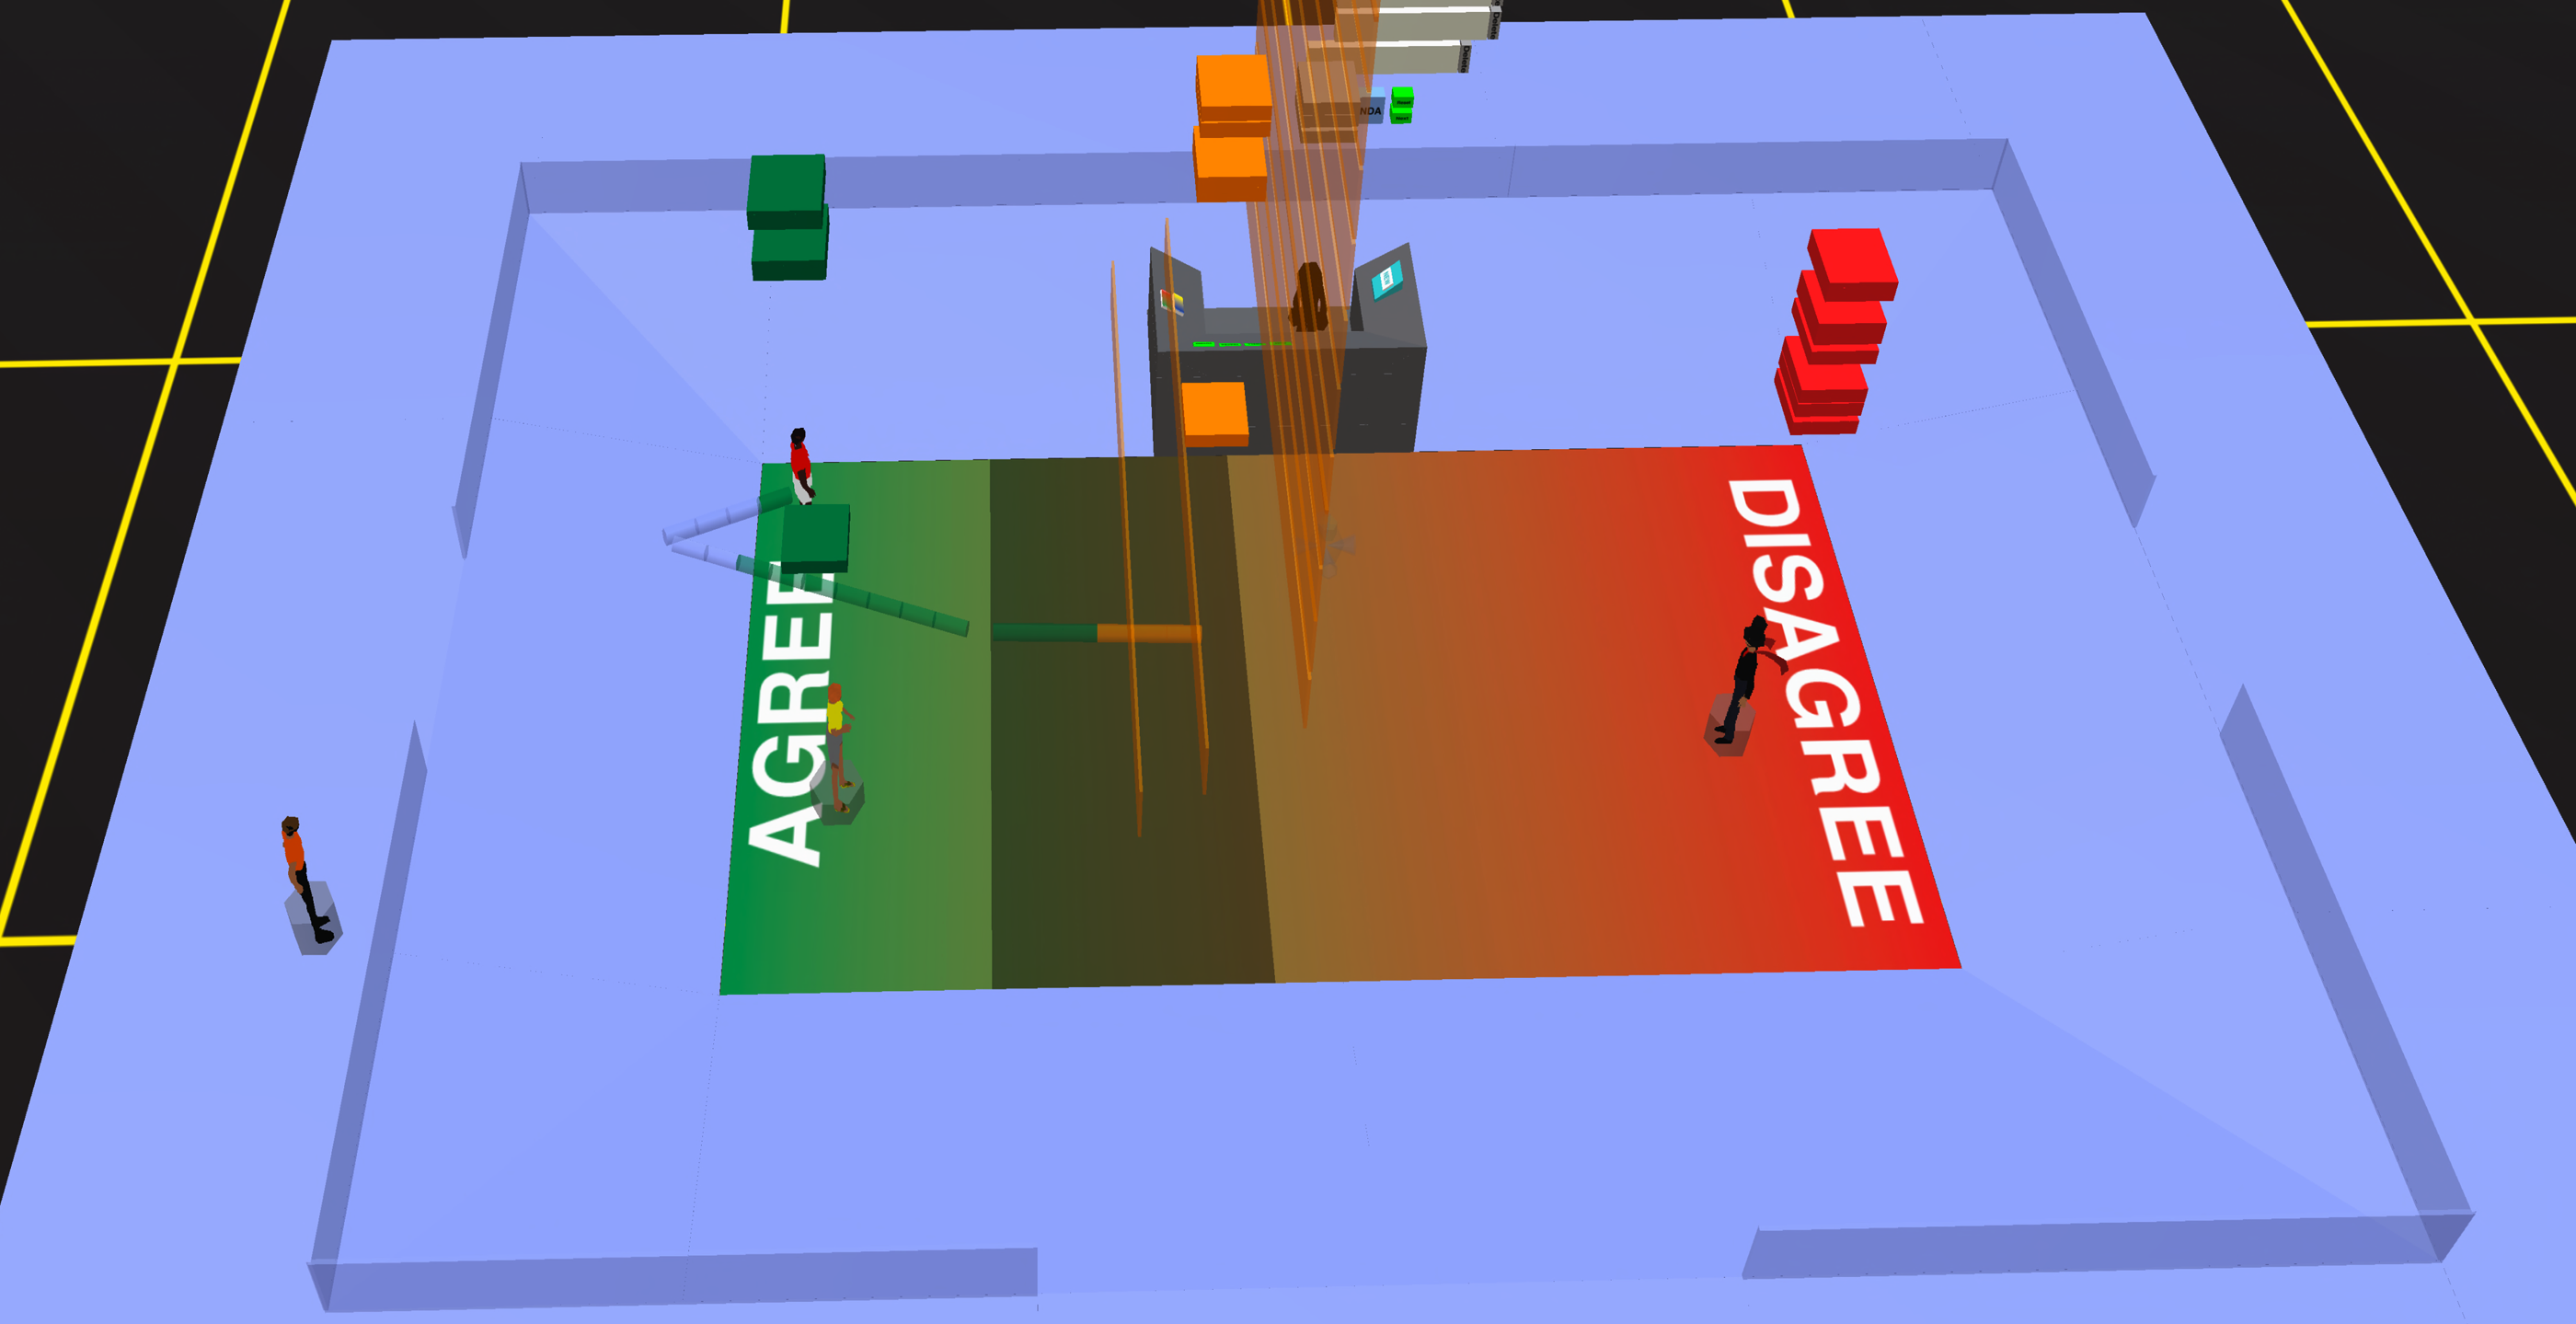
\includegraphics{figures/information-spaces-overview.png}
	\caption{Screenshot of \emph{Information Spaces} in use, showing all the major features at once.}
	\label{fig:information-spaces-overview}
\end{figure*}

\begin{figure*}[t]
	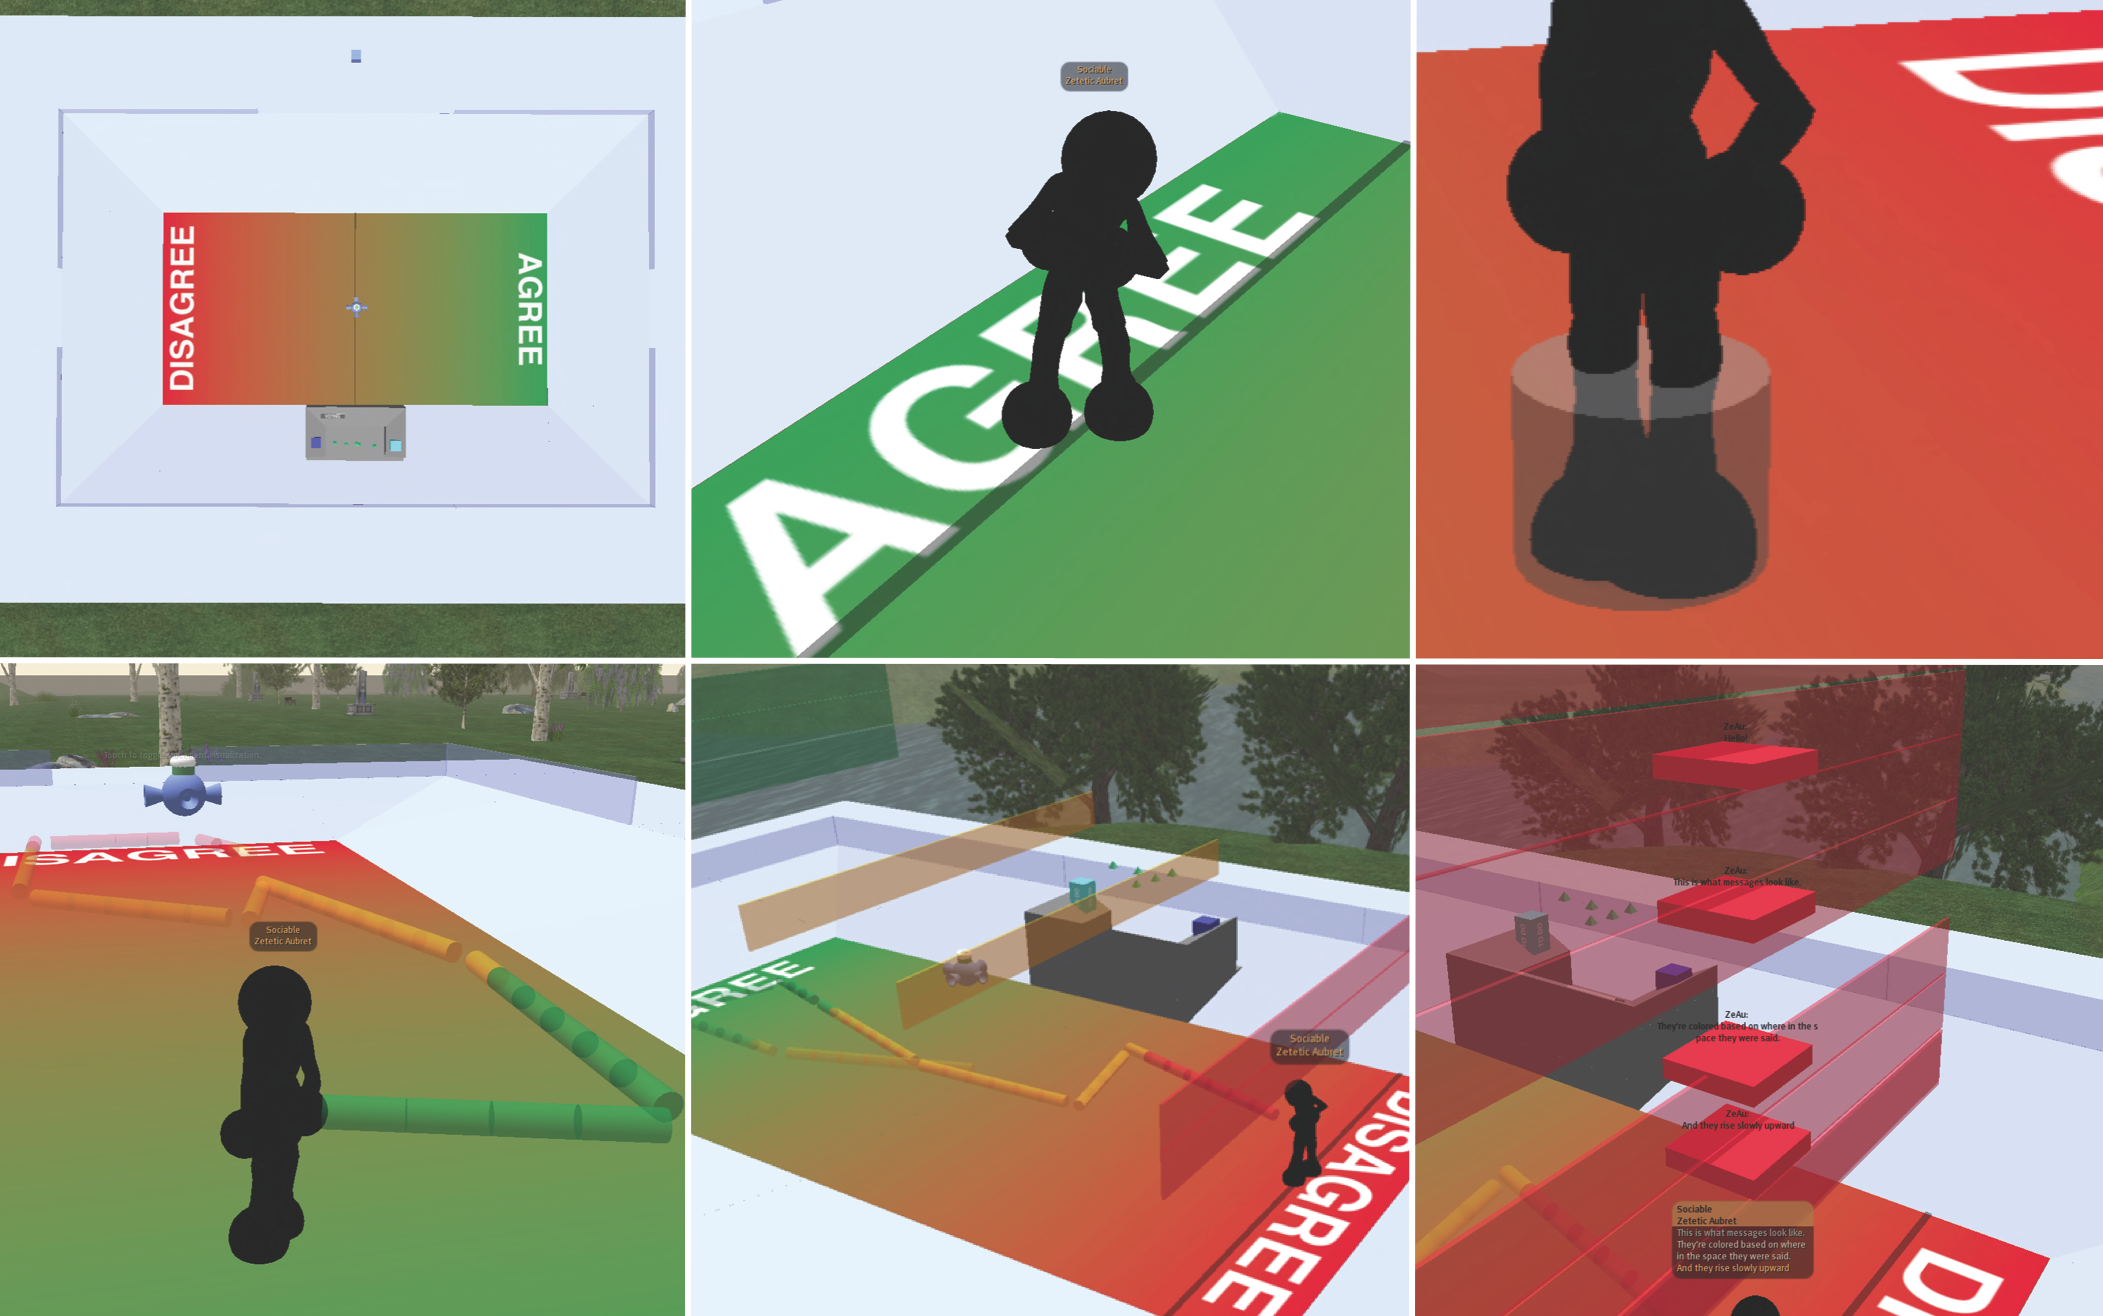
\includegraphics{figures/information-spaces-features.png}
	\caption{Series of screenshots showing each of the major visualizations. Clockwise from upper left: overall layout, average vote indicator, dwell, movement trails, average history, chat history.}
	\label{fig:information-spaces-features}
\end{figure*}


The \emph{Information Spaces} meeting space evokes a very abstract sports stadium. The floor of the field is a colored continuum between ``Agree'' and ``Disagree''. An alternative version of the system used ``Keep Talking'' and ``Move On'' to make the tool useful in discussions that weren't composed of decision-making tasks. Avatars can use their position in the space to indicate how they feel about the decision currently being discussed. Surrounding the colored field is a sloped space, like the stands in a stadium, where avatars can stand and be seen as participants without taking a stand on the issue at hand.

This simple mechanic---where you stand in the space non-verbally communicates your feelings about the meeting---forms a nice foundation for what a virtual meeting room could look like. This is an example of the kind of non-verbal actions that mediated communication can create as an alternative to the subtle face-to-face body language we might have traditionally used to communicate our attitude. It uses the physical form of the space to communicate how it's supposed to be used, without recreating the architecture of a traditional meeting room. The problem is that movements in this space are ephemeral, as they would be face-to-face. If we want someone's position to be meaningful, we must highlight salient features of avatar movement like movement without the space, who's speaking, how long someone has stood somewhere, and so on. \emph{Information Spaces} provides these features through in-context visualizations that reflect people's non-verbal actions back to themselves and others. 


These different social utilities are summarized in figure \ref{fig:information-spaces-features}. When avatars stand still, a dwell indicator appears underneath their avatar which grows slowly the longer they don't move. This helps show avatars who are either fixed in their positions on a discussion question, or who might be idle; other visualizations help disambiguate between those two states. When an avatar moves, their dwell indicator shrinks slowly, and their path is mapped out with a transparent trail. Combined, these visualizations can tell simple stories about someone who had long disagreed on a point and then was swayed and shifted to being in the middle after a particularly convincing argument was made. On the gradient floor, the average position of avatars on the floor is displayed, to demonstrate a sort of visual consensus. In the space above the meeting room, this average is recorded over time by bars that float slowly up above the meeting room. Much like individual movement is recorded by trails on the meeting room floor, the history of the group average feeling is recorded by these floating bars in the sky. Chat messages are recorded similarly. Each time an avatar talks, a small box appears above them and floats up with the average vote bars. This history of the meeting helps participants reflect on meeting process by showing, similar to \citep{DiMicco:2007ie}, relative participation. It adds to that work by also showing a person's location in the space where they were talking, which effectively adds socially significant metadata to the participation visualization.

These visualizations contribute to my main research themes in a number of ways. By not relying on face-to-face techniques for communicating agreement or disagreement \sidenote{More on questions of representational technique and metaphor can be found in \citep{Harry:2008tg}, \citep{Harry:2007cm}, and \citep{Harry:2008vx}. This is a subtle issue, and although in general I advocate for creating new vocabularies being specifically for mediated contexts, the power of well-chosen existing metaphors should not be discounted.} we can add expressive power to an experience. Furthermore, by using shared visualizations to represent those actions we make salient and persistent the actions of others in a way we cannot in face-to-face contexts. Ideally, this allows conversation participants to more easily discuss patterns in participation, although in our trials the limited fluency of most \emph{Second Life} users diminished the extent to which they could attend to these visualizations, particularly the historical visualizations that float above the space.


% do I need to say anything about evaluation here? or can I just end it here?
% I could do a critique of why virtual worlds aren't effective here, but I kinda don't really feel like I have space for it. 

\subsection{backchan.nl}

Face-to-face encounters, as described in the introduction, have a number of inconvenient biases. One venue where these biases become quite visible is when audiences ask questions of presenters and panelists at conferences. Many people might not be comfortable asking questions in front of an audience; those that do feel comfortable asking questions are often asking questions relevant only to themselves, not to the audience as a whole. Even if someone aspires to ask a question that is relevant to a broad section of the audience, how would they know? Furthermore, people tend to ask questions about the content towards the end of a presentation because it's foremost in their mind; recalling questions they might have had from early in the presentation is difficult.

\emph{backchan.nl} addresses these problems by providing a shared space for asking questions and voting on other people's submitted questions. Votes can be either positive or negative. The top eight questions are projected on a display in the space that is visible to the audience, presenters, and moderators. Audience members submit their questions and votes using a web interface that is accessible on either a traditional web interface or an interface sized for mobile devices. Top questions are determined by a ranking algorithm that rewards recent, positive votes. This makes sure that the top posts view doesn't stagnate over long periods. Figure \ref{fig:backchannl} shows what a \emph{backchan.nl} installation looks like in person, and what the web application looks like on a laptop computer. \sidenote{This work is described at greater length in \citep{Harry:2009jh}.}

\begin{figure*}[t]
	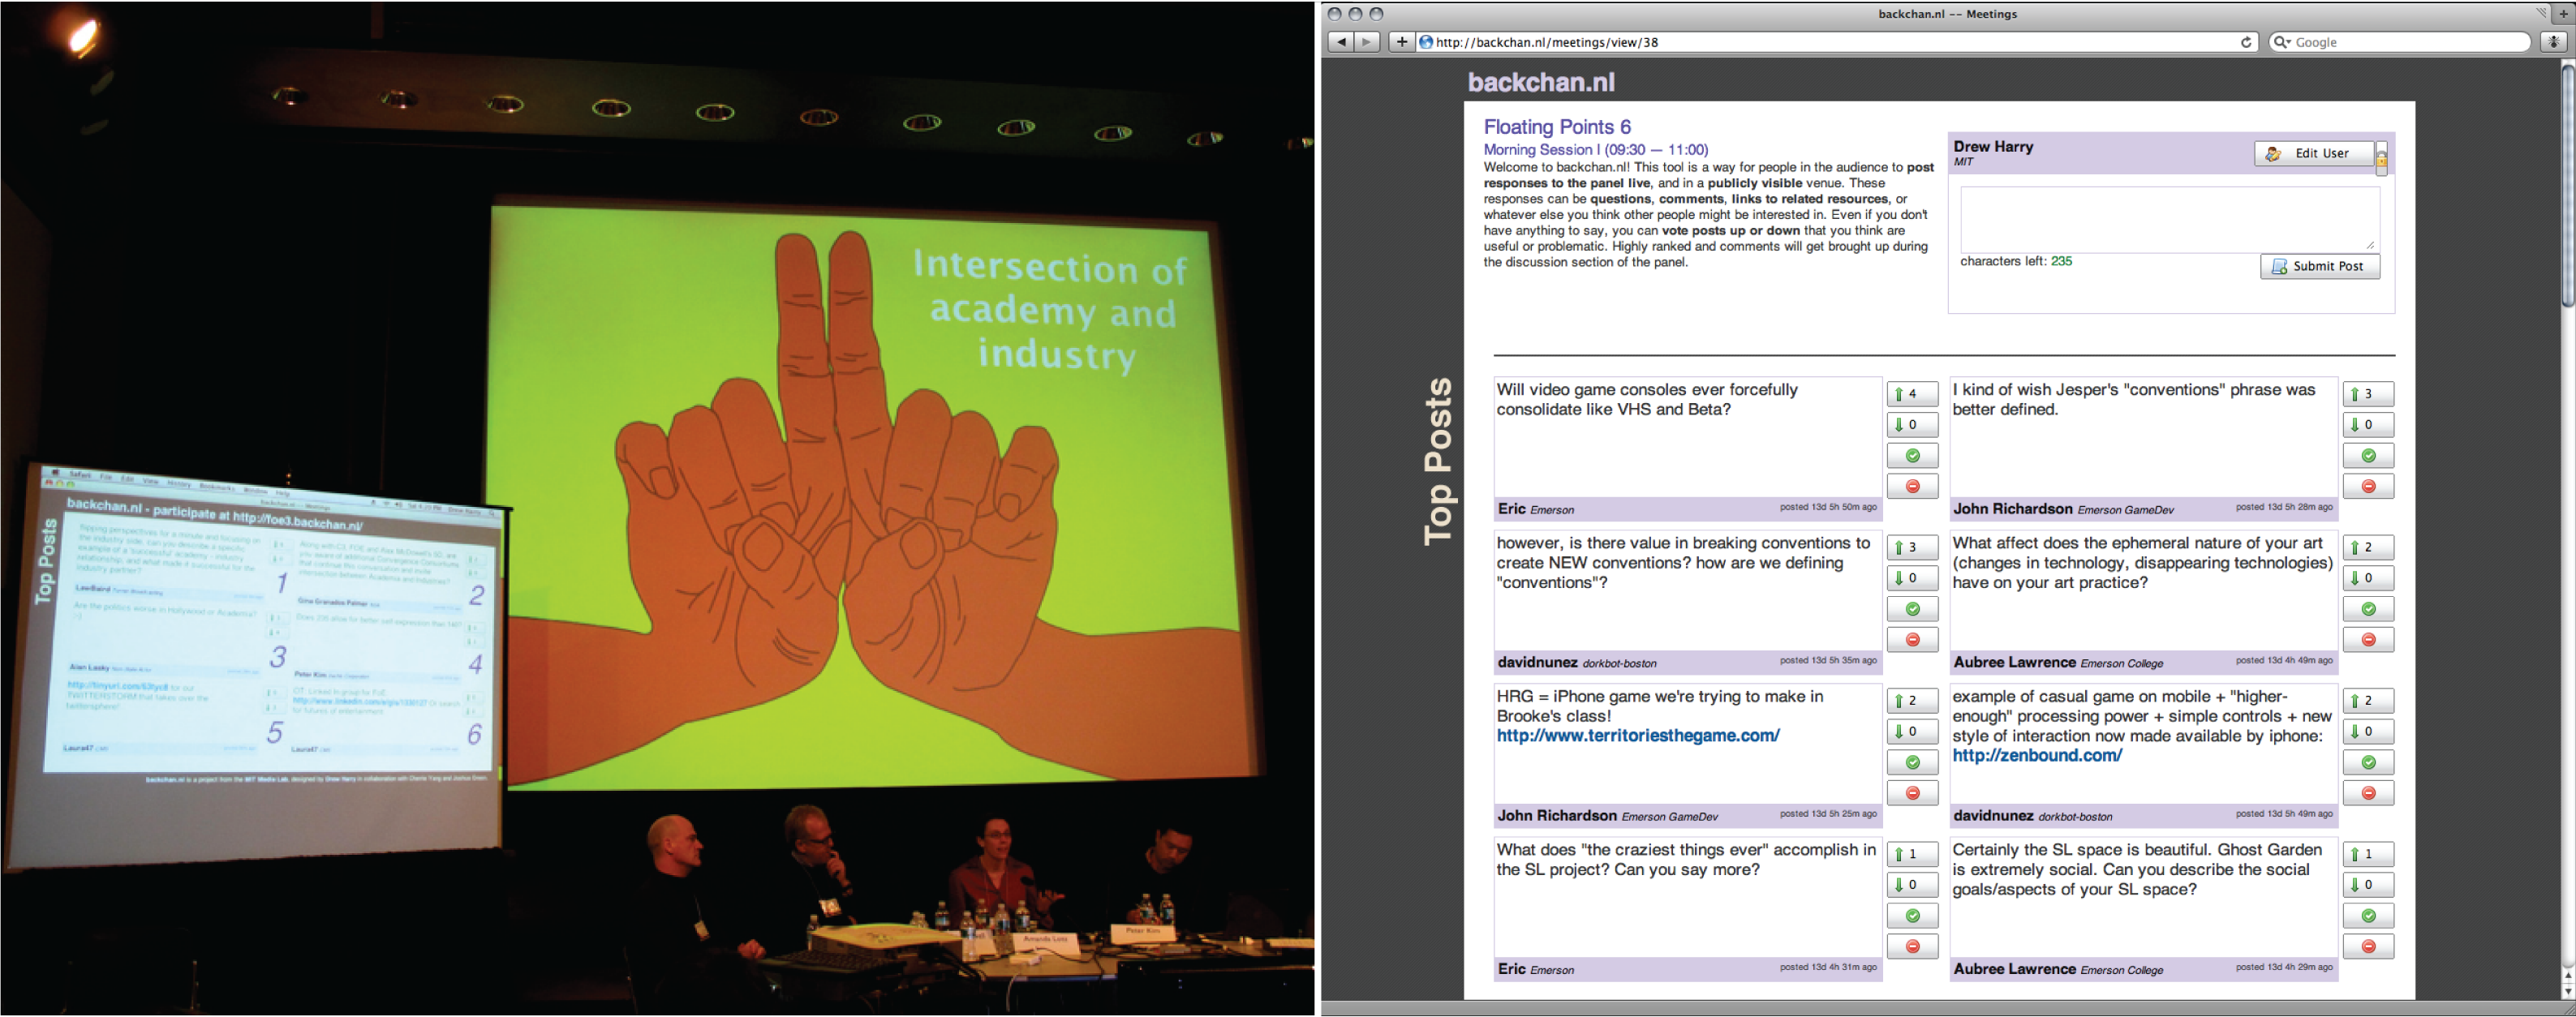
\includegraphics{figures/backchannl.png}
	\caption{Left: Photo of a \emph{backchan.nl} display showing the top audience questions. Right: Screenshot of the full size web interface to \emph{backchan.nl} for posting questions and voting on questions from others.}
	\label{fig:backchannl}
\end{figure*}


Although it was initially designed for a specific panel-based conference, \emph{backchan.nl} has subsequently been deployed in a wide variety of situations. Over the system's almost three year lifetime, more than $400$ events have been created, with over $1200$ meetings. Almost $12000$ unique users have posted or voted in a \emph{backchan.nl} event, creating more than $15000$ posts with almost $60000$ votes. Its broad use has pushed it far beyond its original question-oriented focus. In our study on its use in a pair of early conferences to use \emph{backchan.nl}, we found that although we intended it to be used for questions, it quickly evolved to support content sharing, advertising other backchannels, technical support, as well as communicating about shared issues like temperature, audio problems, or lost items.

My main finding in the \emph{backchan.nl} work was focused on the importance of a shared display to create a space that could promote common ground among audience members and between the audience and presenters. The major problem with past work in this area was, in my view, that backchannels tended to be invisible in the presentation space itself. This led to a number of issues. Conversations tended towards criticism and snarky-ness, not constructive commentary. This is seen most vividly in a Web2.0 Expo talk from danah boyd in 2009 \sidenote{Described from a first person perspective by \citet{boyd:Yo36SNyj}.} and the so-called ``revolt'' at a Mark Zuckerburg interview in 2008\sidenote{Reported after the event in \citep{Wallace:2008vb}. }. With \emph{backchan.nl}, I found this sort of discourse was quite rare and when it did occur it tended to be voted down quickly. The grounding created by the shared display was also important for created a sense of shared space that made it a useful venue for non-question activities like advertising. 

Issues around attention are also clearly at play with this work. Presenters using \emph{backchan.nl} for the first time are frequently less than excited about the presence of another communication channel in a presentation space that they feel a sense of ownership over. This work can also help illuminate how presenters and audience members think about and manage their attention during these kinds of experiences.

% this is a little weak, but I don't really have time for a big discussion here. Plus, attention wasn't a focus of the work originally. If I want to really nail attention in a backchan.nl context, I might need to go back and do some more work with backchan.nl next year. Mention it in future work?


\subsection{Tin Can Classroom}


The physically co-located small group discussion is often viewed as the gold standard for effective collaboration and communication.  It can provide a space for participants to voice their opinions and can readily lead to deliberation and collective problem solving \citep{Burkhalter:2002vg}. \emph{Tin Can Classroom} \sidenote{Parts of the writing in this section were written in collaboration with Prof. Eric Gordon as part of a conference paper submission currently in press. Prof. Gordon was also closely involved with the analysis and study design, as well as some of the design process.} applies the unique properties of a technological system to the established affordances of a small group discussion. We would not deny that face-to-face interaction offers many substantial benefits when compared to interactions mediated by, for instance, a video conferencing system; nevertheless, we argue that there is room to improve the physically proximate small group discussion by intervening in the assumed normal frameworks of turn-taking and attention.

\begin{figure*}[t]
	\includegraphics{figures/tin-can-classroom.png}
	\caption{Left: Screenshot of the tablet interface for \emph{Tin Can Classroom}. Right: Photo of the in-classroom configuration.}
	\label{fig:tin-can-classroom}
\end{figure*}


The \emph{Tin Can Classroom} interface is focused on sharing ideas between students and the professor. Figure \ref{fig:tin-can-classroom} shows the system in use in a classroom, as well as a screenshot of the interface from an in-progress class session. On the right side of the interface is a time-sorted list of submitted ideas. Each idea has its authors name included. When creating an idea, students have the option of placing the idea in the public shared timeline or keeping it in their ``personal'' collection. Around the edge of the interface, each present student's name is shown. Clicking on that student reveals a collection of their personal ideas. Personal ideas can be dragged by anyone into the public idea timeline. This serves as an endorsement and a promotion, and the person who dragged the idea is listed as part of the idea's attribution. The system also helps keep track of conversation topics on the left side of the interface. In this particular class, the student who was running the discussion for the class session would prepare these discussion topics in advance and would manage transitions between them. The time spent on each topic is visualized on an analog clock in the center of the interface. At the end of each class session, all the participants are emailed with a record of the ideas and topics covered in the class session.

To evaluate \emph{Tin Can Classroom} we deployed it to a pair of sections of a media studies graduate seminar classroom for half a semester. Each student, as well as the professor, had their own tablet running the application. In total, the system was used for about $22$ hours of class time with $19$ students. I was present for many of the classes to observe how the system was used. I collected extensive process traces from students' use of the system, and interviewed most of the students at the end of the class.

We found that the presence of a text-based communication system offered a number of major advantages over traditional face-to-face-only class experiences. Most importantly, some students felt empowered to use \emph{Tin Can Classroom} who tended not to participate verbally. We also found that although a lack of confidence was part of why people frequently chose not to participate verbally, we also found that students were hesitant to influence the flow of verbal conversation, but the fluid nature of text-based communication drew broader participation that influenced verbal participation.

This work engages with all three of my main research themes. In our initial research we focused primarily on attention issues, describing how students conceived of attention, chose different channels for different kinds of ideas, and managed their performances on each channel. Our analysis also focused on how promotion---the most important non-verbal action in \emph{Tin Can Classroom}---was interpreted and used by students and the professor. Finally, we observed that although everyone had a tablet with the application running on front of them, we rarely saw students assume that events that were visible on the tablet were already part of the discussion's common ground. Instead, students were frequently prompted by each other or the teacher to re-present their non-verbal contributions verbally to make them part of the verbal discussion. This is either another kind of conversational promotion move that plays a role in demonstrating support for a student's non-verbal contribution, or perhaps a clue that matching private displays are somehow less effective than a fewer number of shared public displays.

% \section{Channels in Practice: Tin Can}
% 
% My final projects exploring the design of backchannels focuses on using tablets to support small group discussion and decision making in face-to-face and distributed contexts. As with my past projects, \emph{Tin Can} is not designed to be a primary communication channel. It coexists with either face-to-face communication or an audio or video conferencing tool. I have created two variants of this tool for different contexts. The first version, called \emph{Tin Can Classroom} is designed to support small group discussions  in a face-to-face classroom context where everyone has their own tablet. The second version, called \emph{Tin Can Conference} is designed for business meetings with mixed groups of remote and local participants, where each location has their own tablet. These projects tie together the major themes of attention, signaling, and grounding that emerged from my previous projects


\section{Tin Can Conference}

The final project in this series is \emph{Tin Can Conference}. Much like \emph{Tin Can Classroom}, it is a tablet-based application designed to support a meeting being conducted using another communication channel. In this case, it is designed to co-exist with an audio or video conferencing system. Unlike the classroom variant, in this system each participant doesn't necessarily have their own tablet (although the system supports that mode, too) but each meeting location has one or more shared tablets that sit between all the participants. The aim with this configuration is to flexibly support a wide range of meeting configurations ranging from everyone being in one room to a meeting with a few people in multiple locations. This kind of heterogeneity reflects the reality of meetings for many people, and is not easily supported by desktop-only designs (embodied by tools like WebEx) or systems that rely on elaborately constructed and specialized rooms (embodied by systems like Cisco's Telepresence Rooms).

Mediated communication channels have a number of important downsides relative to their face-to-face alternatives. Broadly speaking, the latency and low audio quality in most mediated communication challenges tend to add friction to turn-taking, making it difficult to negotiate turns \citep{Brennan:1991wk}. This tends to inhibit the kinds of rapid turn-taking that is critical for people to acknowledge a presentation of information in traditional grounding models in conversation \citep{Clark:1989uc}. In particular, this makes repairing misunderstandings costly. The other major problem faced by mediated meetings is a distinct lack of presence of remote participants. Meeting participants are frequently muted for long periods of a meeting, making it easy for people sharing a physical space to forget there are remote participants. This makes it particularly difficult to judge the engagement and interest of non-speaking participants. The \emph{Tin Can Conference} project seeks to address these issues by creating new kinds of non-verbal actions that both remote and local participants can use to help create a shared record of the meeting, as well as help address some of these larger issues about presence by using tablets as shared displays.

% todo cite some of the major room-oriented design projects that are crazy expensive? don't have those citations at my fingertips.

% talk about the non-duplex-ness of audio communication and the challenges with talking. cite the second grounding paper for that, that lays out the properties. Also think about citing that elsewhere, too.  DONE

\emph{Tin Can Conference} is a shared meeting memory for three major meeting components: tasks, topics, and time. It also reminds meeting participants who is present in the meeting by showing all meeting participants around the edge of the interface. The system provides ways for meeting participants to record these meeting components in the system quickly and easily using either the shared tablets in the room, their own personal tablets, mobile devices, or laptops. These actions are then displayed on all the tablets in the meeting, grounding the conversation with a sense of what's happening in the meeting and where it's going next.

When someone in the meeting brings up a task that needs to be done, anyone in the meeting can feel free to enter it into the system. Recorded tasks are shown on the right side of the interface. At this point, tasks have no owners - they are simply public tasks that can be claimed. Any participant can tap and drag a task to one of the people around the edge of the interface to assign that task to this person. This non-verbal action could be a way for someone to actively claim the task without having to take a speaking turn, or it could reflect someone verbally claiming a task and the actor on \emph{Tin Can Conference} is simply updating the system to reflect the state in the room. Tasks can be dragged back to the shared pool or dragged between meeting participants as well. The number of tasks each participant has assigned is shown as a set of small tabs above their name, making it easy to see at a glance how much work has been assigned to each participant.

The system also helps keep track of meeting topics. As with tasks, they can be entered on any device either during the meeting or in advance. These serve as as a kind of collaboratively constructed agenda. During the meeting, topics can be started and stopped to reflect the current topic being discussed. These actions are made visible to participants in a number of ways. The current topic is always shown at the top of the interface. The clock in the center of the interface helps keep track of how time is being spent on different topics. It shows the current time, while also sweeping out in colored bands that how much time has been spent on the current and past topics. This visualization of how time is spent serves to ground people's notions of the progress of the meeting. Without a visual reminder (as in Second Messenger \citep{DiMicco:2007ie}), it is easy for participants to lose track of time and relative participation.

Activity in \emph{Tin Can Conference} serves two simultaneous purposes. The first order goal is clear: to give meeting participants a shared space to collaboratively construct a sort of annotated meeting record that can be made available to them after the meeting. It is our hope, though, that the vocabulary of non-verbal actions offered by the system also helps to address the larger engagement and acknowledgement issues that occur frequently in distributed meetings. These actions give remote participants a way to signal positive engagement in the meeting. One could not appropriate create a new task object or assign it if they were not engaged with the meeting process. Thus these actions serve as index signals of engagement to other participants who might otherwise assume that their lack of verbal participant means a lack of engagement.



\subsection{Evaluation}

Studying systems like \emph{Tin Can Conference} posts a number of challenges. Modern HCI evaluation is generally focused on lab studies with participants recruited for a single session. This kind of evaluation is simply not effective for addressing my research themes because many of the processes at work in meetings are very difficult to recreate in a lab setting. On the design level, I am interested in understanding how the system is appropriated and what practices develop around its use. Laboratory studies inhibit this process because they inscribe agency on study participants by telling them how they should use the system and making clear both in implicit and explicit ways what kind of behavior is desired. This makes it difficult to make any claims about authentic user practice.

Furthermore, in my past work it has become evident that a group's failure to appreciate a system the first time they use it is not at all predictive of their long-term feelings about the system. This is most clearly evident for \emph{backchan.nl} installations. Nearly every first session of a conference using \emph{backchan.nl} involves a certain amount of hand-wringing from participants about \emph{backchan.nl}'s lack of conversational features, lack of integration with \emph{Twitter}, and a variety of other shortcomings. Yet, after a few sessions of use most critics have come around and report appreciating the tool. Although initial condition issues are widely recognized in the literature, studies are rarely designed to explore the consequences of long term use. It is central to my evaluation efforts to avoid the trap of drawing conclusions from people's single experiences with \emph{Tin Can Conference}.

Creating an evaluation strategy that allows for long-term use in authentic contexts with a group of users who both know each other and have real work to conduct using the system poses a number of challenges. While we were able to achieve this for the \emph{Tin Can Classroom} study, there are some differences in the way we will evaluate \emph{Tin Can Conference}. The primary difference is that I am hoping to deploy the system in a corporate context with a work group that holds frequent distributed meetings and is willing to stick with the tool for a number of sessions both to provide opportunities for analytical insight into how their practices change over time, as well as time to iterate on the design of the system itself. As in the \emph{Tin Can Classroom} study, I hope to be present for these meetings, although this is proving to be a somewhat contentious point with some potential study participants. Similarly, I hope to collect process traces from the meetings, but in a corporate context this kind of data collection can be viewed as somewhat threatening. After the completion of a set of meetings using \emph{Tin Can Classroom} I will interview participants to explore both the impact of the design itself and my primary research themes of non-verbal actions, grounding, and attention.



\section{Research Plan}

Much of this work has already been completed. The three past projects, \emph{Information Spaces}, \emph{backchan.nl}, and \emph{Tin Can Classroom} are done and written up. Most of the engineering for the final project, \emph{Tin Can Conference}, has been completed, although there will undoubtedly be non-trivial work in adapting the system in response to deployment experiences.

The last major hurdle is deploying \emph{Tin Can Conference}. I'm in the process of getting COUHES approval for the experimental part of the work. Simultaneously, I'm working to recruit corporate partners to let me deploy the system in an authentic work context. Three different companies have expressed interest, and I'm working (albeit slowly) to get them to commit to a plan that is close enough to my desired evaluation to be a useful research venue, as well as a plan that is palatable given their various internal constraints. Once the study starts rolling, it will last for a month or two, depending on how many test events I can negotiate for.

After collecting data, the bulk of the remaining work is analysis and writing. Depending on deadlines, I may try to publish the \emph{Tin Can Conference} work separately first, and then fold that writing into the dissertation itself as a way to front-load the work. Indeed, for each of these projects (except \emph{Tin Can Conference}) a publication-quality document has either already been published or is in press, which will ease the dissertation writing process.

There is quite a bit of flexibility in how I spend my remaining time. I hope as part of this proposal process to identify any glaring holes in the overall arc of the work. Although I almost certainly don't have time to do a full new project from scratch, it may make sense to return to an earlier project and consider a different aspect of it; \emph{backchan.nl} might be a particularly appropriate project to re-study in light of how I'm framing my work now. Alternatively, I might spend more time writing with my collaborator on \emph{Tin Can Classroom} from an educational perspective, or do a brief and un-evaluated small final project. It is also possible that setting up an authentic environment to test \emph{Tin Can Classroom} ends up taking up far more time than expected (indeed, it has already taken far longer than I had expected to get this far) and that pushes everything else back.



\subsection{Timeline}

The timeline laid out below is quite rough. Much of this work will be happening in parallel, but it is useful, at least, to list the major milestones between now and graduating even if the dates are relatively loose.

\vspace{1em}
% \begin{table}[t]
\begin{tabular}{ll}
\toprule
Date & Task \\
\midrule

August				& Setup \emph{Tin Can Conference} study \\
August				& Edit CSCW \emph{Tin Can Classroom} paper \\
August/September	& Proposal defense \\
September/October	& Run \emph{Tin Can Conference} study \\
November 			& Analyze \emph{Tin Can Conference} data \\
December			& Outline dissertation \\
Spring				& Write dissertation \\
April				& Draft dissertation to committee \\
May 				& Defend dissertation \\
May					& Submit dissertation \\
\bottomrule

\end{tabular}

% \label{tab:timeline}
% \caption{Broad outline of the remaining tasks and when they will be completed.}
% \end{table}


\bibliography{proposal}
\bibliographystyle{plainnat}


\end{document}
